\documentclass[a4paper]{article}

\usepackage{graphicx}
\usepackage[tuenc]{fontspec}
\usepackage{xcolor}

\usepackage[hidelinks]{hyperref}
\usepackage{csquotes}
\usepackage[english]{babel}
\usepackage[
    backend=biber,
    sorting=none
]{biblatex}

\setmainfont{CMU Serif}
\setlength{\parskip}{\baselineskip}

% Bibliography
\addbibresource{lliurable.bib}

    
\begin{document}

\begin{titlepage}
    \centering
	\vspace{1.5cm}
	{\huge \textbf{\textsc{Unlock the potential of medical imaging data using deep learning}} \par}
	\vspace{2cm}
	{\Large \textit{Joan Marcè i Igual}\par}
	\vfill
    Director: Dr.Benjamin \textsc{Haibe-Kains}
    
    \vfill

    
\includegraphics[width=0.2\textwidth]{images/logo_upc}\par\vspace{1cm}
	\vfill
    
    % Bottom of the page
    {\LARGE Universitat Politècnica de Catalunya \par}
    {\LARGE 2018 \par}
\end{titlepage}

\tableofcontents

\section{Context}

\subsection{Problem formulation}

Nowadays one of the most extensive uses of computing is artificial intelligence. This is being
used from helping us to select what products we can buy based on our preferences to properly detect
faces when taking a picture and focus the camera accordingly. The main advantage of this field is
that once it's working it can continue to work without human intervention.

One of the domains that has greatly increased during the last years is \emph{Machine Learning}.
The main advantage is that it can solely learn from explicit examples without
teaching, and thus reducing the human interaction during the learning process. One of the most used
types is \emph{deep neural networks} and these have demonstrated impressive performance against
task like the classification of digit from the MNIST data set
~\cites{MNIST}{empirical-evaluation-deep-architectures}.

Regarding the medical field, deep learning algorithms, specially convolutional networks, have 
rapidly become the chosen method. These are being used to analyze medical images for tasks such as
image classification, object detection, segmentation and registration among other tasks. This
approach started in the late 1990s and has slowly shifted from systems that are completely designed
by humans to systems that are trained by computers using example data
~\cite{survey-deep-learning}.

To use all this data Survival Prediction models have been created. This type of models are
used to understand the relations between patients and effectiveness of various treatment options. 
The survival and hazard functions are the two fundamental functions in survival analysis. The
survival function \( S(t) = \Pr(T > t) \), is the probability that an individual has
\emph{survived} beyond time \( t \). The hazard function is a measure of risk at time \( t \).
The hazard function \( \lambda(t) \) is defined as:
~\cite{DeepSurv}
\[
    \lambda(t) = \lim_{\delta \rightarrow 0}
    \frac{\Pr(t \le T < t + \delta | T \ge t)}{\delta}
\]


Also, to compare if an algorithm is performing better than another one we usually use the ROC curve
example which compares the \emph{False Positive Rate} against the \emph{True Positive Rate},
see \autoref{fig:ROC-curve}. The Cox Proportional Hazards (CPH) model provides a starting point for a 
survival model and the future models will be compared against this one.
~\cites{ROC-precision-recall}{Cox}

\begin{figure}
    \centering
    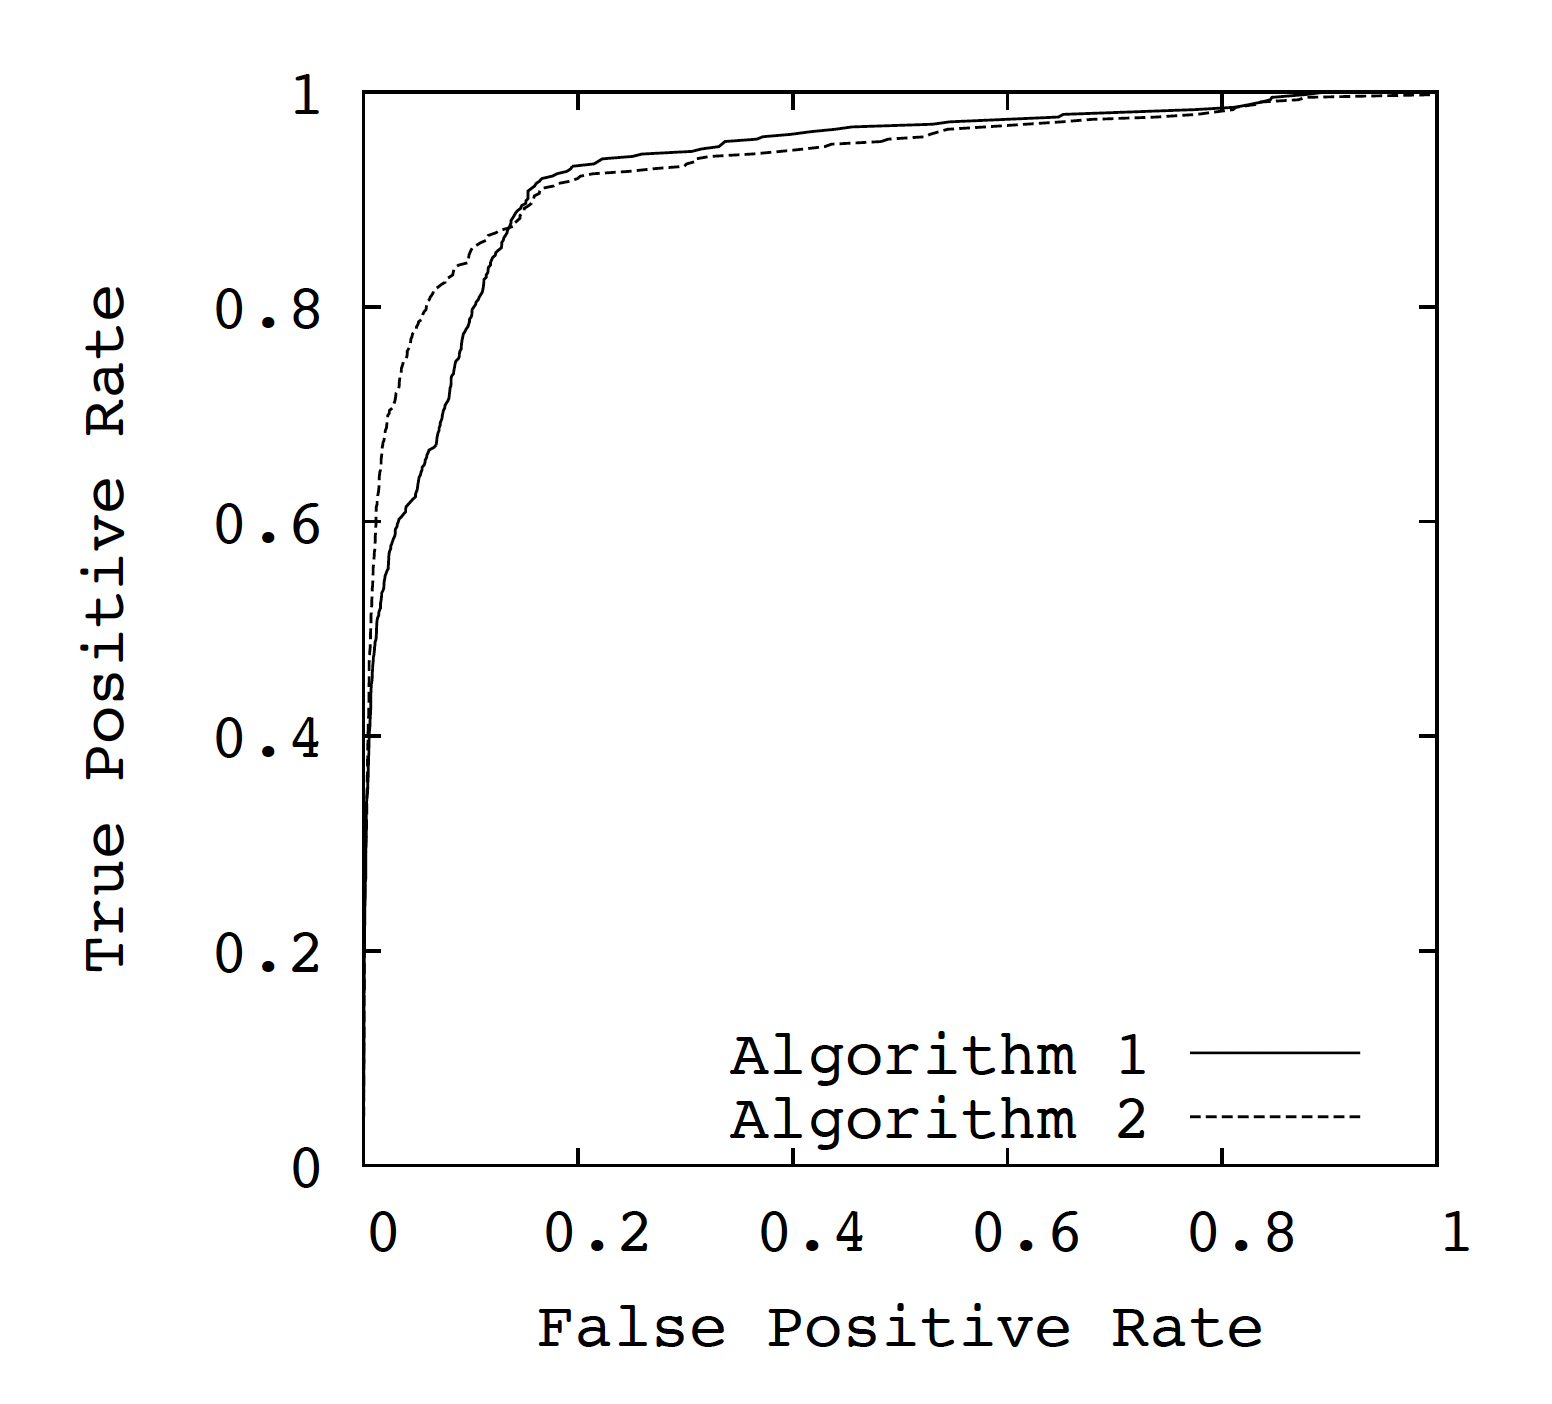
\includegraphics[width=.5\linewidth]{images/roc_curve}
    \caption{ROC Curve example\label{fig:ROC-curve}}
\end{figure}

The objective of this project is to apply the current known methods to create a model for prediction
of survival in head and neck cancer patients. The model should be able to determine the survival


The main objective of this project is to try to apply the current known methods, like DeepSurv, 
for survival prediction and create a 

\subsection{Stakeholders}

\subsubsection{Developer}
\subsubsection{Physicians and Hospitals}
\subsubsection{Patients}

\section{State-of-the-art}

\section{Scope}

\pagebreak
\printbibliography{}

\end{document}